\section{Problem 6: Sommerfeld Model}

\subsection{Results}

\subsubsection{Numerical and Analytical Heat Capacity}
%
The numerical and analytical Sommerfeld heat capacities are shown in Fig. (\ref{sommerfeld_heat_capacity}). Across the temperature range displayed, there is obvious disagreement between the numerical and analytical heat capacities.
\begin{figure}[h]
    \centering
    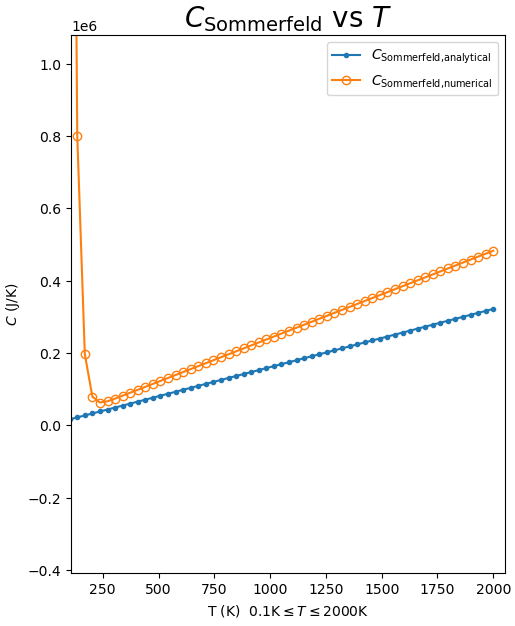
\includegraphics[width=10cm]{sommerfeld_heat_capacity.png}
    \caption{Numerical and Analytical Sommerfeld Heat Capacity vs Temperature}
    \label{sommerfeld_heat_capacity}
\end{figure}
\begin{table}[h]
\begin{center}
    \begin{tabular}{|c|c|c|}
        \hline
        \textbf{System Parameter} & \textbf{Value} & \textbf{Notes} \\ \hline
        Lower Integral Limit & 1 J & - \\ \hline
        Upper Integral Limit & 1$\times 10^{-17}$ J & arbitrary \\ \hline
        No. of Energy Grid Points & 2000 & arbitrary \\ \hline
        Finite Difference Magnitude ($\Delta T$) & 0.001 K & arbitrary \\ \hline
    \end{tabular}
\end{center}
\caption{System Parameters for Fig. (\ref{sommerfeld_heat_capacity})}
\label{system_parameters_for_sommerfeld_heat_capacity}
\end{table}




\subsection{Discussion}

The Sommerfeld model gives a linear relationship between heat capacity and temperature that is valid at low temperatures. The Sommerfeld model shows that this linear relationship may be linked to free electrons obeying Fermi-Dirac statistics in the material.